%!TEX root = ../../Main.tex
\graphicspath{{Chapters/Project/}}
%-------------------------------------------------------------------------------

\chapter{Project}

The project for this reading course is chosen to be carried out using the deep learning framework Caffe. The framework is well known in the deep learning community. It is a rather simple way to obtain a classification convolutional neural network in a very short time, which is the reason why it has been chosen.

The idea of this project is to try out some different neural networks with different values for it's hyperparameters and to see which values will obtain the highest accuracy when training and testing on the CIFAR-10 image data set.

The convolutional network used for inspiration is the one introduced in "Alex's CIFAR-10 tutorial, Caffe style"\footnote{http://caffe.berkeleyvision.org/gathered/examples/cifar10.html} provided by the team behind Caffe. This convolutional network and the changes made to it will be described later on in this chapter along with the architecture and the different types of layers.

\section{Caffe} % (fold)
\label{sec:caffe}

Convolutional Architecture for Fast Feature Embedding (Caffe) is a public available framework which makes it possible to design, train and use a convolutional in a rather simple way. The source code is available online and the team behind the framework encourage other people to note or change any errors which they might find. The framework allows you to choose to use either the CPU or the GPU for calculations. In this project the CPU is used.



In order to use Caffe for image classification three files are needed - a .prototxt file, a \_solver.prototxt file and a .caffemodel file. These three files together defines the architecture of the network, the hyperparameters and the training and testing strategy.

The .caffemodel file defines the architecture of the model e.g. the number and types of layers. An example of a defined layer is shown in

The .prototxt file defines ...

The \_solver.prototxt file defines ...


% section caffe (end)

\section{Convolutional Network architecture} % (fold)
\label{sec:convolutional_network_architecture}

A convolutional neural network exists of a number of different layers with different properties. The different layers used in the networks in this project are described in this section. 

\subsection{Convolutional layers} % (fold)
\label{sub:conv_layers}

The convolutional layers are often the first layers in the network.

Der skal nok skrives lidt om her ..

The rectified Linear Unit (ReLU) is one of many activation function to choose among. The ReLU activation function is the most common activation function in the lower layers of convolutional neural netorks. Other activation functions could be the Sigmoid or the Tanh activation functions.

The ReLU differs from the other mentioned activations function in several ways. First of all it converges faster which results in shorter training time. Second of all the ReLU activation function do not saturate which avoids the problem about the gradient getting killed which would lead to the case where the network stops learning during the training (HENVIS TIL MATERIALE OM AKTIVERINGS FUNKTIONER). This problem is known from the use of the other activation functions. 

The formula for the ReLU activation function is $f(x)=max(0,x)$ and is illustrated in FIGURE..

INDSÆT FIGUR

% subsection conv_layers (end)

\subsection{Pooling layers} % (fold)
\label{sub:pool_layers}

% subsection pool_layers (end)

\subsection{Fully-Connected Layers} % (fold)
\label{sub:fc_layers}

% subsection fc_layers (end)

% section convolutional_network_architecture (end)

\section{Training and testing} % (fold)
\label{sec:training_and_testing}

De forskellige hyperparametre, regularization, mini ba, epoches, 

% section training_and_testing (end)

\section{The networks} % (fold)
\label{sec:the_networks}

\subsection{The original network} % (fold)
\label{sub:the_original_network}

Beskrivelse af arkitekturen og implementationsfilerne

Beskrivelse af resultaterne

% subsection the_original_network (end)

\subsection{Another network} % (fold)
\label{sub:another_network}

Beskrivelse af arkitekturen og implementationsfilerne

Beskrivelse af resultaterne

% subsection another_network (end)

% section the_networks (end)

\section{Results} % (fold)
\label{sec:results}

Sammendrag af alle resultater

\vspace{3 mm} % add some space above the table
\begin{table}[H]
\centering
\sffamily
\small
\begin{tabular}{l | c r}
\toprule
Name 			& Column heading 1 		& Column heading 2	\\
\midrule 
Cell text 	& Cell text					& Cell text			\\ 
Cell text 	& Cell text 				& Cell text 		\\ 
Cell text 	& Cell text 576				& Cell text			\\ 
\bottomrule 
\end{tabular}
\caption[Short caption]{Long caption}
\label{table:table lable}
\end{table}

% section results (end)

\section{Discussion} % (fold)
\label{sec:discussion}

% section discussion (end)

\section{Conclusion} % (fold)
\label{sec:conclusion}

% section conclusion (end)



Here is an inline equation $f(x) = ax+b$. 

\begin{figure}[H]
\centering
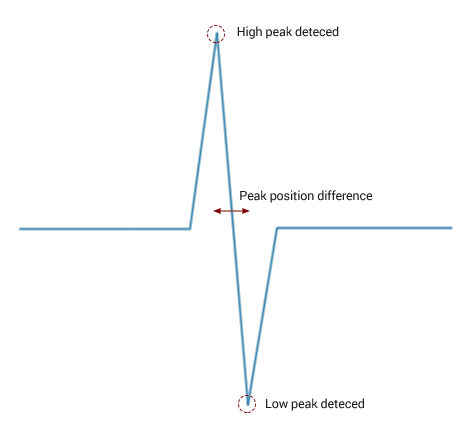
\includegraphics[width = 300 pt]{Img/Figures.png}
\caption{Block diagram}
\label{fig:BlockDiagram}
\end{figure}

\begin{equation}
\frac{n!}{k!(n-k)!} = \binom{n}{k}
\label{eq: myequation}
\end{equation}